\documentclass[10pt,a4paper,french,titlepage]{article}
\author{par Léo Peyronnet}
\title{Jeu du Sokoban\\[1ex] \large Projet Programmation Avancée}
\date{Janvier 2023}

\usepackage{babel}
\usepackage{amssymb}
\usepackage{amsfonts}


\usepackage{xcolor}
\usepackage{listings}

\definecolor{ao(english)}{rgb}{0.0, 0.5, 0.0}

\lstset{
  basicstyle=\footnotesize,
  extendedchars=true,
  framexleftmargin=16pt,
  framextopmargin=3pt,
  framexbottommargin=6pt,
  frame=tb,
  commentstyle=\color{ao(english)},
  breaklines=true,
  keywordstyle=\color{blue},
  language=C,
  literate=
  {²}{{\textsuperscript{2}}}1
  {⁴}{{\textsuperscript{4}}}1
  {⁶}{{\textsuperscript{6}}}1
  {⁸}{{\textsuperscript{8}}}1
  {€}{{\euro{}}}1
  {é}{{\'e}}1
  {è}{{\`{e}}}1
  {ê}{{\^{e}}}1
  {ë}{{\¨{e}}}1
  {É}{{\'{E}}}1
  {Ê}{{\^{E}}}1
  {û}{{\^{u}}}1
  {ù}{{\`{u}}}1
  {â}{{\^{a}}}1
  {à}{{\`{a}}}1
  {á}{{\'{a}}}1
  {ã}{{\~{a}}}1
  {Á}{{\'{A}}}1
  {Â}{{\^{A}}}1
  {Ã}{{\~{A}}}1
  {ç}{{\c{c}}}1
  {Ç}{{\c{C}}}1
  {õ}{{\~{o}}}1
  {ó}{{\'{o}}}1
  {ô}{{\^{o}}}1
  {Õ}{{\~{O}}}1
  {Ó}{{\'{O}}}1
  {Ô}{{\^{O}}}1
  {î}{{\^{i}}}1
  {Î}{{\^{I}}}1
  {í}{{\'{i}}}1
  {Í}{{\~{Í}}}1,
}

\usepackage{tikz}
\usetikzlibrary{automata, arrows.meta, positioning,shapes}

\begin{document}
\maketitle
\tableofcontents
\newpage
\section{Du jeu en tant que concept}
\subsection{Rappel des règles du jeu}
Sokoban est un jeu de puzzle dans lequel le joueur doit pousser des caisses sur des cibles. Voici comment le jeu fonctionne:
\begin{itemize}
\item Le joueur peut se déplacer dans quatre directions: haut, bas, gauche, droite.
\item Le joueur doit pousser les caisses sur les cibles, mais il ne peut pousser qu'une caisse à la fois et ne peut pas tirer une caisse.
\item Les caisses ne peuvent être poussées que sur des espaces vides ou sur des cibles. Elles ne peuvent pas être poussées contre des murs ou d'autres caisses.
\item Le joueur doit utiliser sa stratégie et ses habiletés de résolution de problèmes pour déplacer toutes les caisses sur les cibles dans le niveau le plus efficacement possible.
\item Le jeu se termine lorsque toutes les caisses ont été déplacées sur les cibles ou lorsque le joueur abandonne.
\end{itemize}

\subsection{Modélisation du jeu}
À partir de ces règles, nous avons du faire des choix arbitraires pour la représentation des différents concepts que prend en compte le jeu:
\subsubsection{Terrain/Carte}
Pour modéliser le terrain de jeu, nous avons fait le choix de l’afficher dans le terminal avec les symboles suivants : 
\begin{itemize}
\item Les murs sont représentés par le symbole “{\#}”.
\item Les caisses sont représentés par la lettre “O”.
\item Les cibles sont représentés par la lettre “x”.
\item Les caisses se trouvant sur une cible sont représentés par le chiffre “0”.
\item Le joueur est symbolisé par la lettre “P”.
\end{itemize}
\subsubsection{Contrôles du personnage}
Pour pouvoir déplacer le personnage sur le terrain dans les quatre directions possibles, nous avons choisi les contrôles suivants :
\begin{itemize}
\item Déplacement vers le haut: touche h.
\item Déplacement vers le bas: touche b.
\item Déplacement vers la gauche: touche g.
\item Déplacement vers la droite: touche d.
\end{itemize}
L'utilisateur a également la possibilité d'abandonner à tout moment la partie, il lui suffit de rentrer la lettre 'a' dans le terminal.
\newpage
\section{Au programme informatique}
\subsection{Structuration des données}\label{struct}
Maintenant que les éléments du jeu sont modélisés, il faut les structurer en données compréhensible pour un ordinateur. Nous allons donc utiliser la fonctionnalité "struct" du langage C afin de regrouper plusieurs éléments/variables proches sémantiquement dans un même objet.
\subsubsection{terrain}
Un terrain de jeu de Sokoban pour être représenté par un tableau à deux entrées. Ainsi, en C, nous inclurons dans notre structure "terrain" un pointeur de pointeurs de caractères dans le but d'allouer dynamiquement un tableau 2D plus tard dans le programme. 

Afin de délimiter la taille de ce tableau, nous ajoutons également à cette structure deux entiers représentant le nombre de lignes et de colonnes que devra faire le tableau. 

Cette structure possède également un dernier entier correspondant au nombre de cibles présentes sur le terrain.
Nous avons donc:
\begin{lstlisting}
typedef struct terrain terrain;
struct terrain{
    char ** data;
    int nbLigns;
    int nbCols;
    int nbCibles;
};
\end{lstlisting}
\subsubsection{perso}
Notre structure "perso" regroupe l'ensemble des variables définissant le personnage jouable sur le terrain. Ainsi, elle possède une paire d'entiers permettant de déterminer respectivement sur quelle ligne et sur quelle colonne du terrain se trouve notre personnage. 

Elle possède également un troisième entier $\in \{0,1\}$(booléen) permettant de savoir si le personnage se trouve sur une cible ou non. Cet entier se justifie par le fait que notre modélisation ne comprend pas de caractère pour le cas où le personnage se trouve sur une cible (cela aurait pu être "R" par exemple). Nous avons donc:
\begin{lstlisting}
typedef struct perso perso;
struct perso{
int lign;
int col;
short int surCible;
};
\end{lstlisting}
\subsubsection{partie}
Enfin, nous avons fait le choix de regrouper nos deux structures définies ci-dessus dans une ultime structure "partie". Elle possède donc un pointeur vers une structure "terrain" et un autre pointeur vers une structure "perso". Ces pointeurs seront alloués à l'initialisation d'une partie.

La structure "partie" possède également un pointeur de caractères qui permettra que garder en mémoire le nom de la partie. Elle possède également un entier "puntos" indiquant le nombres de cibles couvertes par une caisse. Nous avons donc:
\begin{lstlisting}
typedef struct partie partie;
struct partie{
    terrain *terrain;
    perso *perso;
    int puntos;
    char *nom;
};
\end{lstlisting}
\subsection{Structure du programme}
Un code source bien structuré permet une meilleure lisibilité du code. Ainsi, comme pour les données, nous avons décidé de regrouper les morceaux de notre code ayant une sémantique proche dans des fichiers sources (.c) différents et de les relier avec des fichiers en-tête (.h).
\begin{itemize}
\item struct.h: possède l'ensemble du code présenté dans la partie \ref{struct}.
\item affichage.c: possède le code des fonctions d'affichages.
\item partie.c: possède le code de la fonction partieSokoban(). (c.f. \ref{partie})
\item main.c: possède le code de la fonction main().
\end{itemize}
Ces différents codes sources sont reliés comme suit:
\begin{figure}[h]
\centering
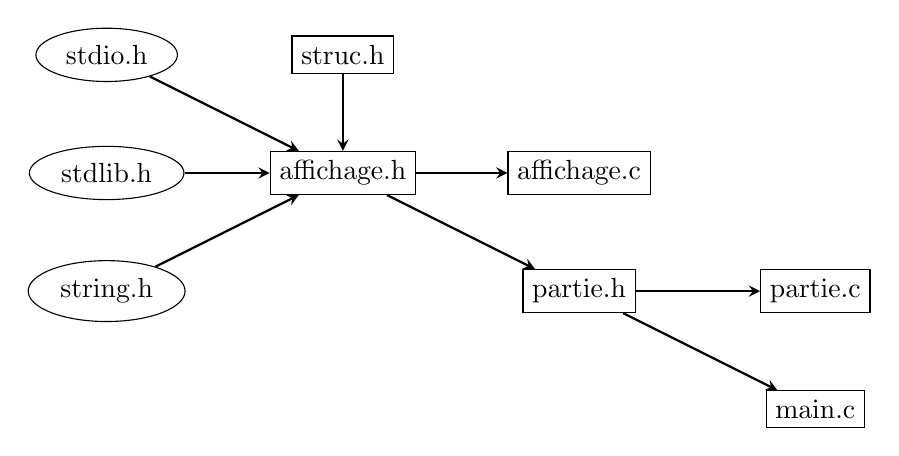
\begin{tikzpicture} [node distance = 3cm, on grid, auto]
\node (0) [rectangle,draw] {struc.h};
\node (1) [rectangle,draw, below=1.5cm of 0] {affichage.h};
\node (2) [rectangle,draw, right = of 1] {affichage.c};
\node (3) [rectangle,draw, below = 1.5cm of 2] {partie.h};
\node (4) [rectangle,draw, right = of 3] {partie.c};
\node (5) [rectangle,draw, below = 1.5cm of 4] {main.c};
\node (6) [ellipse,draw, left = of 0] {stdio.h};
\node (7) [ellipse,draw, below = 1.5cm of 6] {stdlib.h};
\node (8) [ellipse,draw, below = 1.5cm of 7] {string.h};
 
\path [-stealth, thick]
    (0) edge  node  {} (1)
    
    (1) edge  node {} (2)
    (1) edge  node {} (3)
    
    (3) edge node {}  (4)
    (3) edge  node {}  (5)
    
    (8) edge node {}  (1)
    (7) edge node {}  (1)
    (6) edge node {}  (1);
\end{tikzpicture}
\caption{Diagramme de l'organisation des fichiers}
\end{figure}

stdio.h, stdlib.h et string.h sont des librairies de fonctions standards du langage C, aucun package n'est à pré-installer pour lancer notre programme.
\newpage
\subsection{Fonctions d'affichage}
\subsubsection{fonction afficher\_ascii\_art()}
Cette fonction va prendre en argument un pointeur sur une chaine de caractère constante. Elle aura pour effet de bord d'afficher le contenu du fichier qu'on lui passe en argument.
\begin{lstlisting}
void afficher_ascii_art(const char *nom_fichier) {
    FILE *fp;
    int c;
    fp = fopen(nom_fichier, "r");
    if (fp == NULL) {
        perror("Erreur lors de l'ouverture du fichier");
        return;
    }
    while ((c = fgetc(fp)) != EOF) {
        putchar(c);
    }
    fclose(fp);
}
\end{lstlisting}
\textit{Tout d'abord elle va initialiser une variable “fp” qui va être de type FILE * et un entier “c”. Ensuite elle va ouvrir le fichier qu’on lui a mis en argument en lecture et assigner ce fichier a fp. Si l'ouverture du fichier ne s’exécute pas correctement, fp sera égal à “NULL” et la fonction affichera alors “Erreur lors de l'ouverture du fichier”. Si le fichier s'ouvre correctement, la boucle while va affecter un à un chaque caractère du fichier à “c” et va l'afficher tant que “c” est différent de EOF c’est a dire “END OF FILE” qui est la fin du fichier. Enfin, la dernière ligne de cette fonction va refermer le fichier ouvert.}
\subsubsection{fonction texte\_encadre()}
Cette fonction va prendre en argument un pointeur sur une chaine de caractère constante et un entier. Elle aura pour effet de bord d'afficher une ligne de “=” avec au milieu de cette ligne le mot mis en argument.
\begin{lstlisting}
void texte_encadre(const char * mot, int bande){
    bande=(bande-strlen(mot)-2)/2;
    for (int i=0;i<bande;i++){
        printf("=");
    }
    printf(" ");
    printf("%s",mot);
    printf(" ");
    for (int i=0;i<bande;i++){
        printf("=");
    }
    printf("\n");
}
\end{lstlisting}
\textit{La première ligne va modifier la valeur de la variable bande, elle va tout d'abord enlever la longueur du mot moins 2 à la valeur de bande. Ensuite, elle va diviser la valeur du nombre obtenu par 2. La boucle for va afficher un “=” tant que i est strictement inférieure à la valeur de bande et va s'incrémenter de 1 à chaque tour de la boucle. Cela va donc former une bande de “=”. La fonction va ensuite afficher un espace, puis le mot mis en argument de la fonction et un espace après le mot. Il y a ensuite, une nouvelle boucle for, identique à la première qui va donc afficher une bande de “=” après le mot. Pour finir la fonction saute une ligne dans le terminal.}
\subsubsection{fonction printMenu()}
Cette fonction ne prend aucun élément en argument, elle a pour effet de bord d'afficher le menu.
\begin{lstlisting}
void printMenu(){
    system("clear");
    afficher_ascii_art("./programme/ressources/sokoban.txt");
    printf("\n");
    printf("\n");
    texte_encadre("MENU",80);
    printf("\t1. Jouer à la partie de test\n");
    //printf("\t2. Jouer au mode histoire\n");
    //printf("\t3. Jouer à une partie enregistée dans un fichier .csv\n");
    printf("\tq. Quitter\n");
    for (int i=0;i<80;i++){
        printf("=");
    }
    printf("\n");
}
\end{lstlisting}
Ce qui donne:
\begin{figure}[h]
\centering
\includegraphics[scale=0.6]{img/menu.JPG}
\end{figure}
\subsubsection{fonction printTerrain()}
Cette fonction prend en argument un terrain t, cette fonction affiche le terrain qu’on lui met en argument. 
\begin{lstlisting}
void printTerrain(terrain *t){
    for (int i=0;i<t->nbLigns;i++){
        for (int j=0;j<t->nbCols;j++){
            printf("%c",t->data[i][j]);
        }
        printf("\n");
    }
}
\end{lstlisting}
\subsection{Fonction partieSokoban()}\label{partie}
La fonction "partieSokoban()" se situe pour rappel dans le fichier "partie.c". Elle prends en argument un pointeur sur une structure "partie", ne renvoie rien et a pour effet de bord la modification des variables suivantes:
\begin{itemize}
\item partie$\rightarrow$terrain$\rightarrow$data
\item partie$\rightarrow$perso$\rightarrow$lign
\item partie$\rightarrow$perso$\rightarrow$col
\item partie$\rightarrow$perso$\rightarrow$surCible
\item partie$\rightarrow$puntos
\end{itemize}
Cette fonction peut se diviser en trois parties/états:
\begin{enumerate}
\item Affichage interface et entrée utilisateur
\item Modification des variables en fonction de l'entrée utilisateur
\item Affichage final (victoire ou défaite)
\end{enumerate}
L'état 1 et 2 alternent en boucle jusqu'à ce qu'une condition de fin de partie soit remplie. Alors, l'algorithme passe en état 3 puis se termine. Il y a deux conditions de fin de partie: une en cas de victoire et une en cas de défaite. La condition de victoire est remplie lorsque l'entier "puntos" est égal à l'entier "nbCibles". La condition de défaite est remplie lorsque l'utilisateur abandonne. Elles sont codées à la ligne 23, en tant que condition d'une boucle while.
\subsubsection*{État 1}
L'état 1 correspond au code de la ligne 13 à 21 lors du premier input de l'utilisateur puis de la ligne 117 à 126 jusqu'à la condition de fin de jeu. Après l'affichage du nome de la partie et du terrain, l'utilisateur rentre un input censé symboliser un déplacement au l'abandon.
\subsubsection*{État 2}
L'état 2 correspond au code de la ligne 25 à 116. L'input de l'utilisateur est transformé en un vecteur $\vec{v}=(x,y)$.\\
Si l'input de l'utilisateur est égal à:
\begin{itemize}
\item h: $x=0;y=-1$
\item b: $x=0;y=1$
\item g: $x=-1;y=0$
\item d: $x=1;y=0$
\end{itemize}
Sachant que le personnage jouable possède déjà un vecteur $\vec{p}=(lign,col)$ qui correspond à la position du caractère "P" au début de la partie. Sachant que le terrain correspond à une matrice $A=(\{"\mbox{x}","\;","O","0","\#","P"\})_{i,j\in \mathbb{N}^+}$.\\\\
Alors, les règles du Sokoban sont ensuite appliquées selon les cas suivants:
\begin{itemize}
\item $A_{col+x,lign+y}="\;"$: alors, $A_{col,lign}="\;"$ et $A_{col+x,lign+y}="P"$
\item $(A_{col+x,lign+y}="O") \land (A_{col+2x,lign+2y}\in \{"\#","0","O"\})$: \textit{(cf partie.c)}
\item $(A_{col+x,lign+y}="0") \land (A_{col+2x,lign+2y}\in \{"\#","0","O"\})$: \textit{(cf partie.c)}
\item $A_{col+x,lign+y}="\mbox{x}"$: \textit{(cf partie.c)}
\end{itemize}


A la fin de chacun de ces cas de figure, $\vec{p}=\vec{p}+\vec{v}$.\\
\\\\
L'algorithme manipule également l'entier "surCible" en l'incrémentant lorsqu'une cible est remplacée par le caractère "P" puis en le décrémentant lorsque le personnage bouge à nouveau.

\subsubsection*{État 3}
L'état 3 correspond au code de la ligne 129 à 150. L'affichage final diffère en fonction de la condition de fin de partie (victoire ou défaite).

\end{document}